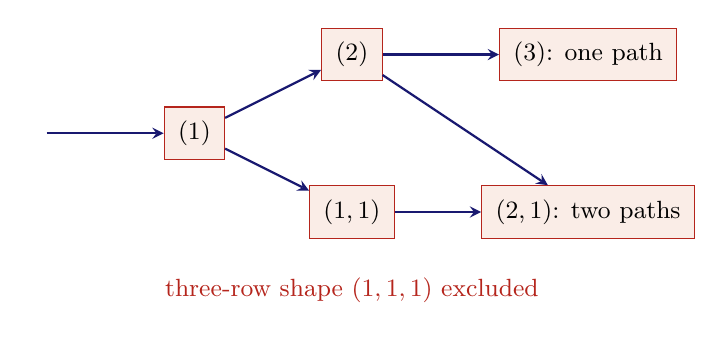
\begin{tikzpicture}[x=1cm,y=1cm,>=stealth,every node/.style={font=\small},edge/.style={->,thick,MidnightBlue}]
\node (empty) at (0,0) {$\varnothing$};
\node[draw=BrickRed,fill=BrickRed!6,inner sep=5pt] (one) at (2,0) {$(1)$};
\node[draw=BrickRed,fill=BrickRed!6,inner sep=5pt] (two) at (4,1) {$(2)$};
\node[draw=BrickRed,fill=BrickRed!6,inner sep=5pt] (eleven) at (4,-1) {$(1,1)$};
\node[draw=BrickRed,fill=BrickRed!6,inner sep=5pt] (three) at (7,1) {$(3)$: one path};
\node[draw=BrickRed,fill=BrickRed!6,inner sep=5pt] (twoone) at (7,-1) {$(2,1)$: two paths};
\draw[edge] (empty)--(one);\draw[edge] (one)--(two);\draw[edge] (one)--(eleven);
\draw[edge] (two)--(three);\draw[edge] (two)--(twoone);\draw[edge] (eleven)--(twoone);
\node[align=center,text=BrickRed] at (4,-2) {three-row shape $(1,1,1)$ excluded};
\end{tikzpicture}
